\PassOptionsToPackage{table,dvipsnames}{xcolor}
%%%%%% PREAMBULE
\documentclass{beamer}

\usepackage[frenchb]{babel}
\usepackage[T1]{fontenc}
\usepackage[utf8]{inputenc}
%\usepackage[table,dvipsnames]{xcolor}
\usepackage{graphicx}
\usepackage{colortbl}
\usepackage{graphics}

\usetheme{CambridgeUS}
% Antibes, Bergen, Berkeley, Berlin, Copenhagen, Darmstadt, Dresden, Frankfurt, Goettingen, Hannover, Ilmenau, JuanLesPins, Luebeck, Madrid, Malmoe, Marburg, Montpellier, PaloAlto, Pittsburgh, Rochester, Singapore, Szeged, Warsaw, boxes, default, CambridgeUS
\usecolortheme{default}
% default, albatross, beaver, beetle, crane, dolphin, dove, fly, lily, orchid, rose, seagull, seahorse, whale, wolverine

\usepackage{hyperref}
\usepackage{fancybox}
\usepackage{multirow}
\usepackage{cases}
\usepackage{hyperref}

\usepackage[table,dvipsnames]{xcolor}
\usepackage[sort&compress,numbers]{natbib}
\usepackage{apalike}
% \usepackage{cite} % commenter si la biblio est pas générée
\usepackage{verbatim}
\usepackage{amsfonts}
\usepackage{amsmath}
\usepackage{ulem}
\usepackage{mathtools}
\newcommand{\norm}[1]{\left\lVert#1\right\rVert}
\newcommand{\abs}[1]{\left\lvert#1\right\rvert}

\usepackage{adjustbox}
\usepackage{amssymb,latexsym}
\usepackage{mathrsfs}
\usepackage{subfig}
\usepackage{placeins}
\usepackage{float}
\usepackage[bottom]{footmisc}
\usepackage{default}
\usepackage{multicol}

\usepackage{listingsutf8}

\usepackage{mcode}

\renewcommand{\tt}[1]{\texttt{#1}}


%%%%%% DEFINITION D'UN BOOLEEN POUR LE LOGO
\newif\ifplacelogo 
\placelogotrue 
\logo{\ifplacelogo
\includegraphics[height=5mm]{LogoINSA.png}\fi} 

%%%%%% INFORMATIONS GENERALES DU DOCUMENT
\title[Projet TI]{Projet de Théorie de l'Information}
\subtitle{Stéganographie dans les images}

\author[G. Darchen, A. Huat, R. Judic]{Gautier Darchen, Alexandre Huat, Romain Judic}

\institute[]{INSA Rouen\\ASI4}
\date{\today}
%\logo{
\includegraphics[height=5mm]{LogoINSA.png}}

%%%%%%DEBUT DU DOCUMENT
\begin{document}
\placelogotrue	% met le booleen du logo à VRAI

	%%%%%%%%%% PAGE DE TITRE
	\begin{frame}
	\titlepage
	\end{frame}
	
	%%%%%%%%%%%%%%%%%%%%%%%%% SOMMAIRE
	\begin{frame}[label=sommaire]{Sommaire}
		\tableofcontents%[currentsection, hideothersubsections]
	\end{frame}
	
	%%%%%%%%%%%%%%%%%%%%%%%%%% STEGANOGRAPHIE
	\section{Stéganographie}	
	
	%%%%%%%%%%%%%%%%%%%%%%%%%%%%%%%%%%%%%%%%%%%%% Substitution de LSB
	\subsection{Stéganographie par substitution de LSB}
	
	% LSB 1	
	\begin{frame}
	\frametitle{Stéganographie par substitution de LSB (1/5)}
	\begin{alertblock}{Définition}
   	\rightskip=0pt\leftskip=0pt
	\begin{itemize}
	 	\item LSB : \textit{Least Significant Bit}
	 	\item LSB (pixels) de l'image substitués par bits du message à insérer
	 	\item Destinataire connaît le sens de lecture de l'image pour déchiffrer le message
	\end{itemize}
	\end{alertblock}

 
	\begin{exampleblock}{Exemple}
   	\rightskip=0pt\leftskip=0pt
   		{\small
			\underline{Message ($M$) :} $M = 11001000$ \hfill \underline{Stéganographie :} $M$=\textbf{\textcolor{red}{1}
						  \textcolor{blue}{1}
						  \textcolor{green}{0}
						  \textcolor{orange}{0}
						  \textcolor{gray}{1}
						  \textcolor{Brown}{0}
						  \textcolor{RubineRed}{0}
						  \textcolor{Violet}{0}}
		}
		
		{\tiny
		\begin{minipage}{.5\textwidth}\centering
			\begin{tabular}{|c|c|c|c|}
			\hline
			00110100 & 11001010 & 01101001 & 11101101 \\\hline
			10000010 & 10100100 & 00101101 & 10111011 \\\hline
			\end{tabular}
			\captionof{table}{Image originale en niveaux de gris}
		\end{minipage}
		\begin{minipage}{.5\textwidth}\centering
			\begin{tabular}{|c|c|c|c|}
			\hline
			0011010\textcolor{red}{\textbf{1}} & 1100101\textcolor{blue}{\textbf{1}} & 0110100\textcolor{green}{\textbf{0}} & 1110110\textcolor{orange}{\textbf{0}} \\\hline
			1000001\textcolor{gray}{\textbf{1}} & 1010010\textcolor{Brown}{\textbf{0}} & 0010110\textcolor{RubineRed}{\textbf{0}} & 1011101\textcolor{Violet}{\textbf{0}} \\\hline
			\end{tabular}
			\captionof{table}{Image modifiée en niveaux de gris}
			\end{minipage}
		}
	\end{exampleblock}
	\end{frame}
	
	% LSB 2
	\begin{frame}
	\frametitle{Stéganographie par substitution de LSB (2/5)}
	\begin{alertblock}{Programme utilisé}
   	\rightskip=0pt\leftskip=0pt
	\begin{itemize}
	 	\item Code \textit{Matlab}
	 	\item Deux images en entrée :
	 		\begin{itemize}
	 		\item \textit{cover} : image dans laquelle on dissimule un message
	 		\item l'image à cacher
	 		\end{itemize}
	 	\item Transformation des images en niveaux de gris (pixels codés sur un octet)
	 	\item Nombre de bits à substituer choisi par l'utilisateur
	\end{itemize}
	\end{alertblock}
	\end{frame}
	
	% LSB 3
	\begin{frame}
	\frametitle{Stéganographie par substitution de LSB (3/5)}
	\begin{exampleblock}{Application}
   	\rightskip=0pt\leftskip=0pt
	\begin{minipage}{.33\textwidth}\centering
		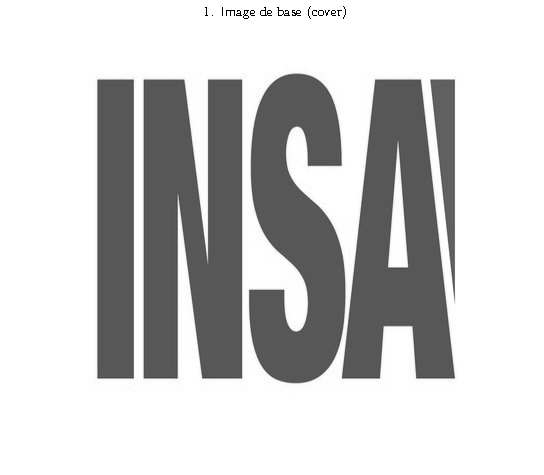
\includegraphics[scale=0.18]{images/fig1.png}
		{\centering\captionof*{figure}{Image de base (\textit{cover})}}
		\label{fig1}
	\end{minipage}
	\begin{minipage}{.32\textwidth}\centering
		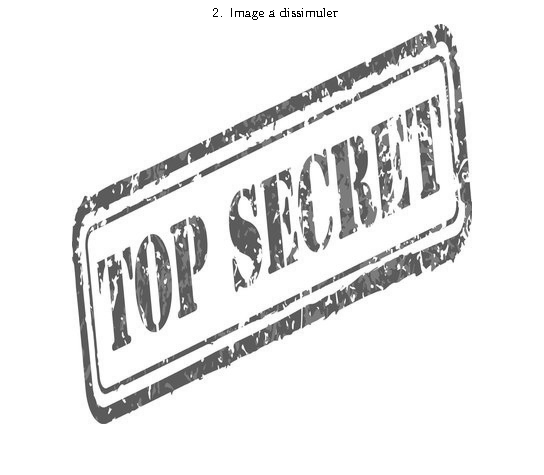
\includegraphics[scale=0.18]{images/fig2.png}
		{\centering\captionof*{figure}{Image à dissimuler}}
		\label{fig2}
	\end{minipage}
	\begin{minipage}{.32\textwidth}\centering
		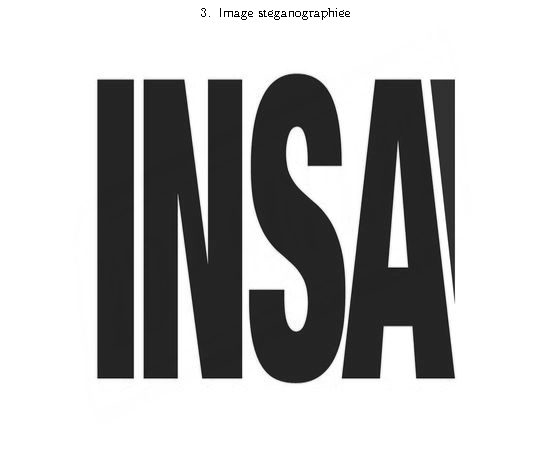
\includegraphics[scale=0.18]{images/fig3.png}
		{\centering\captionof*{figure}{Image stéganographiée}}
		\label{fig3}
	\end{minipage}

	\begin{minipage}{.33\textwidth}\centering
		
\includegraphics[scale=0.18]{images/fig4.png}
		{\centering\captionof*{figure}{Image extraite de la stéganographie}}
		\label{fig4}
	\end{minipage}
	\begin{minipage}{.32\textwidth}\centering
		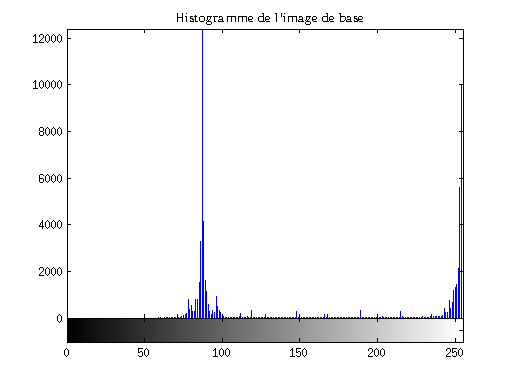
\includegraphics[scale=0.18]{images/fig5.png}
		{\centering\captionof*{figure}{Histogramme de l'image \textit{cover}}}
		\label{fig5}
	\end{minipage}
	\begin{minipage}{.32\textwidth}\centering
		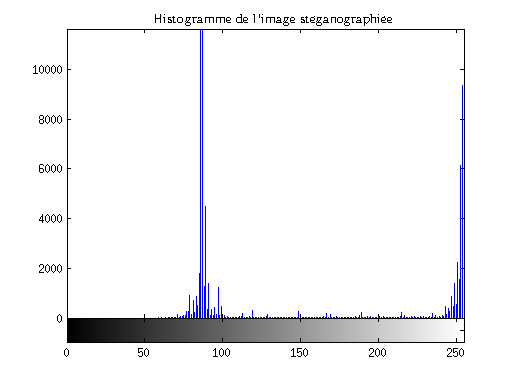
\includegraphics[scale=0.18]{images/fig6.png}
		{\centering\captionof*{figure}{Histogramme de l'image stéganographiée}}
		\label{fig6}
	\end{minipage}
	\end{exampleblock}
	\end{frame}
	
	% LSB 4
	\begin{frame}
	\frametitle{Stéganographie par substitution de LSB (4/5)}
	\begin{block}{Commentaires (1/2)}
   	\rightskip=0pt\leftskip=0pt
	\begin{itemize}
	 	\item Difficile de voir à l'\oe il nu qu'un message est dissimulé
	 	\item Message récupéré sans trop de distorsion
	 	\item $$ EQM = \frac{1}{m\cdot n}\sum_{i=0}^{m-1}\sum_{j=0}^{n-1}\big(I_1(i,j)-I_2(i,j) \big)^2 = 1.39\times 10^4$$
	 		avec \begin{itemize}
	 				\item $I_1$ : l'image originale à dissimuler
	 				\item $I_2$ : l'image dissimulée récupérée après stéganographie
	 				\item $m$ et $j$ : resp. hauteur et largeur des images.
	 			\end{itemize}
	 		L'EQM est relativement élevée car 
	 			\begin{itemize}
	 				\item faible distance entre pixels
	 				\item bit de plus faible poids changé ou non pour chaque pixel
	 				\item[$\implies$] nombre de pixels différent entre les deux images (EQM) élevé
	 			\end{itemize}
	\end{itemize}
	\end{block}
	\end{frame}
	
	
	% LSB 5
	\begin{frame}
	\frametitle{Stéganographie par substitution de LSB (5/5)}
	\begin{block}{Commentaires (2/2)}
   	\rightskip=0pt\leftskip=0pt
	\begin{itemize}
	 	{\footnotesize\item PSNR : \textit{Peak Signal to Noise Ratio}
	 	$$PSNR = 10\cdot \log_{10}\left(\frac{d^2}{EQM}\right) = 10.6027 $$
		avec \begin{itemize}
			\item $d$ : la dynamique du signal $\iff$ valeur maximale qu'un pixel peut avoir
				\begin{itemize}
					\item $d=255$ dans notre cas (pixels codés sur 8 bits)
				\end{itemize}
			\end{itemize}
		\item Histogrammes grossièrement identiques $\iff$ information de chaque pixel peu modifiée}
	\end{itemize}
	\end{block}
	
	\begin{alertblock}{Critique de la substitution de LSB}
   	\rightskip=0pt\leftskip=0pt
   		\begin{description}
   		{\small
   		\item[Avantage] Facile à implémenter et complexité de calculs faible
   		\item[Inconvénient] Facilement repérable et attaquable (attaque du $\chi^2$) car distribution statistique du support altérée
   		}
   		\end{description}
   	
   	\end{alertblock}
	\end{frame}

	
	\subsection{SSIS : Spread Spectrum Image Steganography}
	
	\begin{frame}
	\frametitle{SSIS : Spread Spectrum Image Steganography (1/4)}
	\begin{alertblock}{Définition}
   	\rightskip=0pt\leftskip=0pt
	\begin{itemize}
	 	\item Dissimuler le message dans un bruit de faible puissance et de même dimension (spatiale) que l'image \textit{cover}
		\item Le spectre (fréquentiel) du message est "étalé" $\implies$ ses motifs spatiaux ne sont plus visibles à l'oeil nu
	\end{itemize}
	\end{alertblock}
	\begin{alertblock}{Algorithme - Insertion}
	\begin{enumerate}
		\item Soit un message $m$ (chiffré ou non) et une \textit{cover} $f$
		\item Générer, avec une clé $k$, un bruit pseudo-aléatoire $n$
		\item Étaler spatialement $m$
		\item Moduler le bruit $n$ par le message $m$ $\implies s$
		\item Additionner la \textit{cover} $f$ et le signal $s$ obtenu : $f + s = g$
	\end{enumerate}
	\end{alertblock}
	\end{frame}
	
	\begin{frame}
	\frametitle{SSIS : Spread Spectrum Image Steganography (2/4)}
	\begin{alertblock}{Algorithme - Extraction}
	\begin{enumerate}
		\item Soit $g$ l'image stéganographiée
		\item On calcule une estimation $\hat{f}$ de l'image initiale
		\item On calcule $\hat{s}$ l'estimation de $s$ : $\hat{s} = g - \hat{f}$
		\item On génère à nouveau le bruit $n$ avec la clé $k$
		\item On démodule une estimation $\hat{m}$ du message
	\end{enumerate}
	\end{alertblock}

	\begin{exampleblock}{Exemple : modulation par un bruit}
	\begin{itemize}
		\item[$\rightarrow$] $m$ est une image NB
		\item[$\rightarrow$] $m = $ [1~ -1~ -1~~ 1~~ 1~~ 1~ -1]
		\item[$\rightarrow$] ~$n = $ [a ~~b ~~c ~~d ~~e ~~f ~~g]
		\item[$\rightarrow$] On applique le signe de $m$ sur $n$ :\\~$s = $ [a ~-b ~-c ~~d ~~e ~~f ~-g]
	\end{itemize}
	\end{exampleblock}
	\end{frame}
	
	\begin{frame}
	\frametitle{SSIS : Spread Spectrum Image Steganography (3/4)}
	\begin{exampleblock}{Insertion dans la vraie vie}
		\begin{center}
		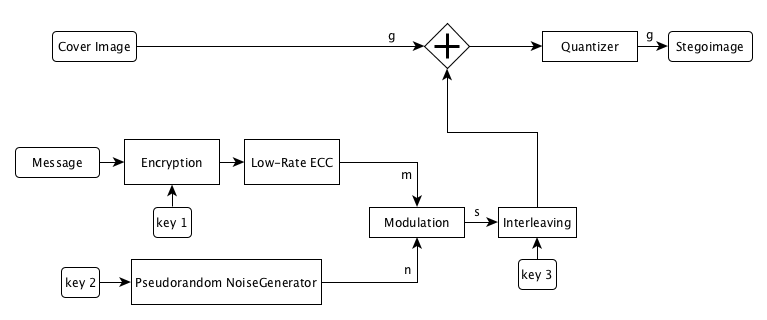
\includegraphics[scale=0.4]{images/SSIS_insert.png}
		\captionof*{figure}{Algorithme d'insertion de l'Army Research Laboratory}
		\label{fig8}
		\end{center}
	\end{exampleblock}
	\end{frame}
	
		\begin{frame}
	\frametitle{SSIS : Spread Spectrum Image Steganography (4/4)}
	\begin{alertblock}{Critique de la méthode Spread Spectrum}
	\begin{description}
		\item[Avantage] Le tatouage est complètement invisible et difficilement décelable par analyse informatique.
		\item[Inconvénient] Besoin d'un décodeur pour estimer l'image \textit{cover} initiale $\implies$ difficile à mettre en place
	\end{description}
	\end{alertblock}
	\end{frame}
	
	
	
	%%%%%% TRANSFORMED DOMAIN STEGANOGRAPHY
	
	% sources
	% https://fr.mathworks.com/help/wavelet/ref/dwt2.html?searchHighlight=dwt2&s_tid=doc_srchtitle
	% http://www-ljk.imag.fr/membres/Valerie.Perrier/PUBLI/Cours2-VP.pdf
	
	\subsection{Stéganographie dans le domaine transformé}
	
	\begin{frame}{Stéganographie dans le domaine transformé (1/5)}
		\begin{alertblock}{Principe}
			Cacher l'information dans le domaine transformé de l'image (domaine fréquentiel au lieu du domaine spatial)
		\end{alertblock}		
		\begin{exampleblock}{Différentes méthodes}
			\begin{itemize}
				\item Jsteg (Derek Upham, 1998) : LSB sur les coefficients de la transformée en cosinus discrète (DCT)
				\item F5 (Westfeld, 2001) : générer des nombres pseudo-aléatoires avec une clé $k$ déterminant quel \textit{chemin} suivre pour l'insertion/extraction des bits dans la DCT puis insertion avec un codage de Hamming.
				\item Utilisation de la \textbf{transformée en ondelettes discrète (DWT)} (démonstration).
			\end{itemize}
		\end{exampleblock}
	\end{frame}
	
	\begin{frame}{Stéganographie dans le domaine transformé (2/5)}
		\framesubtitle{Exemple avec la DWT}
		\begin{block}{La transformée en ondelettes}
			Analogue à la transformée de Fourier : la TF décompose le signal en sinus, la DWT en ondelettes. Une ondelette est une fonction arbitraire $\Phi$ vérifiant :
			$$ \iint_{\mathbb{R}^2} \frac{\abs{\Phi(k)}^2}{\norm{k}^2}dk < +\infty $$
			On génère une famille d'ondelette par dilatation (coef $a$), translation (vecteur $b$) et rotation (angle $\theta$) de l'ondelette mère $\Phi$. D'où la transformée en ondelette :
			$$Wf(a,b,\theta)=\iint_{\mathbb{R}}f(x)\Phi_{(a,b,\theta)}^{*}dx$$
		\end{block}
	\end{frame}

	\begin{frame}{Stéganographie dans le domaine transformé (3/5)}
		\framesubtitle{Exemple avec la DWT : Et en pratique ?}
		\begin{columns}[c]
			\begin{column}{.45\linewidth}
			\begin{figure}[h]
				\centering
				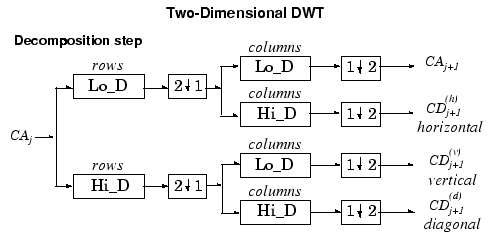
\includegraphics[width=\linewidth]{images/dwt2-decomposition-step.png}
				\caption*{Etapes de décomposition de la DWT}
			\end{figure}
			\end{column}
		
			\begin{column}{.45\linewidth}
			\begin{figure}[h]
				\centering
				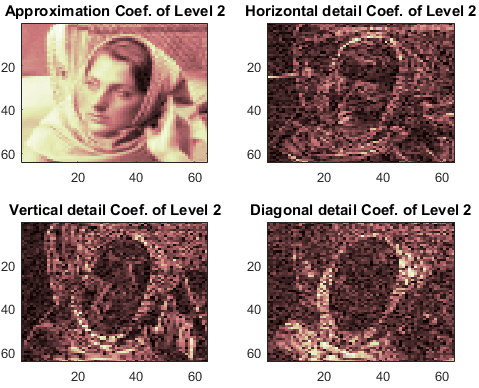
\includegraphics[width=\linewidth]{images/decompo-example.png}
				\caption*{Exemple de décomposition de la DWT}
			\end{figure}
			\end{column}
		\end{columns}
	\end{frame}

	\begin{frame}{Stéganographie dans le domaine transformé (4/5)}
		\framesubtitle{Exemple avec la DWT}
		\begin{block}{Implémentation}
			\begin{enumerate}
				\item Analyser la cover-image (payload, contours), faire des pré-traitements (contraste, luminosité, gamma, etc.).
				\item Calculer la DWT.
				\item Choisir un chemin d'implantation (connu de l'autre partie) : insérer les bits dans les hautes fréquences (i.e. matrices $\neq CA$).
				\item Implanter le message (mix avec une autre technique de stegano possible).
				\item Construire la stego-image (DWT inverse).
				\item Envoyer le message !
			\end{enumerate}
		Pour retrouver le message : faire le chemin inverse évidemment.
		\end{block}
	\end{frame}

	\begin{frame}{Stéganographie dans le domaine transformé (5/5)}
	\framesubtitle{Exemple avec la DWT}
		\begin{block}{Commentaires}
			\begin{itemize}
				\item Robuste à la compression et aux stéganalyses
				\item Faible payload
				\item Reconstruction de bonne qualité
			\end{itemize}
		\end{block}
	\end{frame}
	
	%%%%%%%%%%%%%%%%%%%%%%%%%%
	
	
	
	%%%%%%%%%%%%%%%%%%%%%%%%%% STEGANALYSE
	\section{Stéganalyse}
	
	% Steganalyse 1
	\begin{frame}
	\frametitle{Stéganalyse  (1/5)}
	\begin{alertblock}{Définition (1/2)}
   	\rightskip=0pt\leftskip=0pt
	\begin{itemize}
	 	\item But : détecter si une image est susceptible de contenir des informations dissimulées par stéganographie
	 		\begin{itemize}
	 		\item Identifier les messages suspects
	 		\item Déterminer s'ils contiennent un message caché
	 		\item Et si possible le décoder
	 		\end{itemize}
	 	\item Discipline duale de la stéganographie
	 	\item Difficulté réside dans le fait qu'on ne sait pas si un message est dissimulé ou non
	 	\item Différent de la cryptanalyse où on est sûr qu'un message est caché
	 	\item Si un message est dissimulé, distribution statistique de l'image certainement altérée
	 	\item Problèmes très souvent liés aux distributions statistiques du support des images à analyser
	\end{itemize}
	\end{alertblock}
	\end{frame}
	
	% Steganalyse 2
	\begin{frame}
	\frametitle{Stéganalyse (2/5)}
	\begin{alertblock}{Définition (2/2)}
   	\rightskip=0pt\leftskip=0pt
	\begin{itemize}
	 	\item Il existe 3 types de stéganalyse :
	 		\begin{description}
	 		\item[Stéganalyse passive] Détecter la présence d'un secret.
	 		\item[Stéganalyse active] Détecter puis détruire le secret.
	 		\item[Stéganalyse malicieuse] Détecter le message, comprendre l'algorithme de stéganographie et l'extraire pour ses propres fins.
	 		\end{description}
	\end{itemize}
	\end{alertblock}
	
	\begin{exampleblock}{Stéganalyse d'un message dissimulé par substitution de LSB}
   	\rightskip=0pt\leftskip=0pt
   	\begin{itemize}
   	 	\item Stéganographie invisible à l'\oe il nu
   	 	\item Modification des LSB d'une image $\implies$ variations entre les pixels voisins de l'image
   	 	\item[Si] information dissimulée dans les LSB d'une image
   	 	\item[Alors] histogramme de l'image non uniforme 
   	\end{itemize}
   	\end{exampleblock}
	\end{frame}
	
	% Steganalyse 3
	\begin{frame}
	\frametitle{Stéganalyse (3/5)}
	\begin{exampleblock}{Application à LSB (1/2) (démonstration)}
   	\rightskip=0pt\leftskip=0pt
	\begin{itemize}
	 	\item Message dissimulé sur les bits de poids faibles	
	 	\item[] $\implies$ la parité des pixels est modifiée
	 	\item On parcourt l'image à analyser et on met tous les pixels pairs à 0 (noir en RGB) et tous les pixels impairs à 255 (blanc)
	 	\item Cela met en évidence les pixels modifiés par un possible message caché
	\end{itemize}
	\end{exampleblock}
	\end{frame}
	
	% Steganalyse 4
	\begin{frame}
	\frametitle{Stéganalyse  (4/5)}
	\begin{exampleblock}{Application à LSB (2/2)}
   	\rightskip=0pt\leftskip=0pt
   	\begin{minipage}{.45\textwidth}\centering
		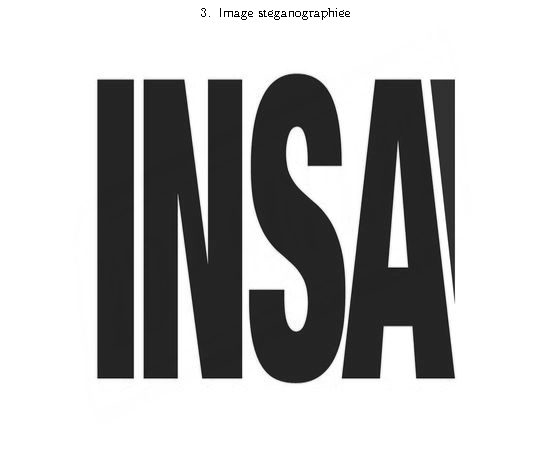
\includegraphics[scale=0.3]{images/fig3.png}
		{\centering\captionof*{figure}{Image à analyser}}
		\label{fig3}
	\end{minipage}
	\begin{minipage}{.45\textwidth}\centering
		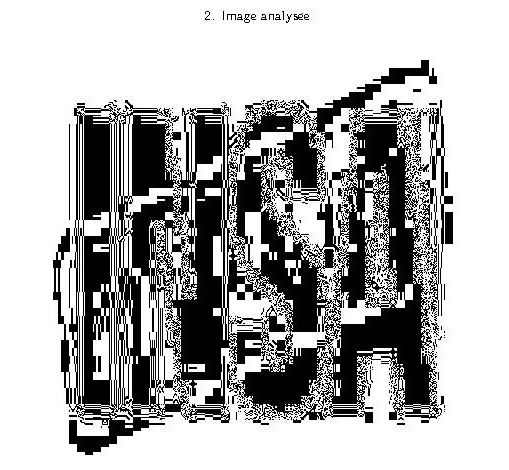
\includegraphics[scale=0.25]{images/fig7.png}
		{\centering\captionof*{figure}{Image révélée}}
		\label{fig8}
	\end{minipage}
	
	\end{exampleblock}
	\end{frame}

	\begin{frame}{Stéganalyse (5/5)}
		\begin{exampleblock}{Détection par machine learning}
			\begin{enumerate}
				\item Obtenir une grande BD d'images.
				\item Séparer les images sur différents ilôts (méthode K-means)
				\item Chaque ilôt est associé à un classifieur (le classifieur décide si l'image est cover ou stego). Classifieur au choix (SVG, Average Perceptron, EFLDFS etc.)
				\item Apprentissage puis test
			\end{enumerate}
		Résultats avec un classifieur EFLDFS : $>95 \%$ de réussite avec 150 000 images !
		\end{exampleblock}
	\end{frame}

	%%%%%%%%%%%%%%%%%% APPLICATIONS


	\section{Applications}
	
	\begin{frame}{Applications}
		\begin{itemize}
			\item Tatouage numérique invisible
			\item Transmission de données confidentielles dans l'industrie nucléaire
			\item Echange de données militaires ou d'espionnage
			\begin{figure}[h]
				\centering 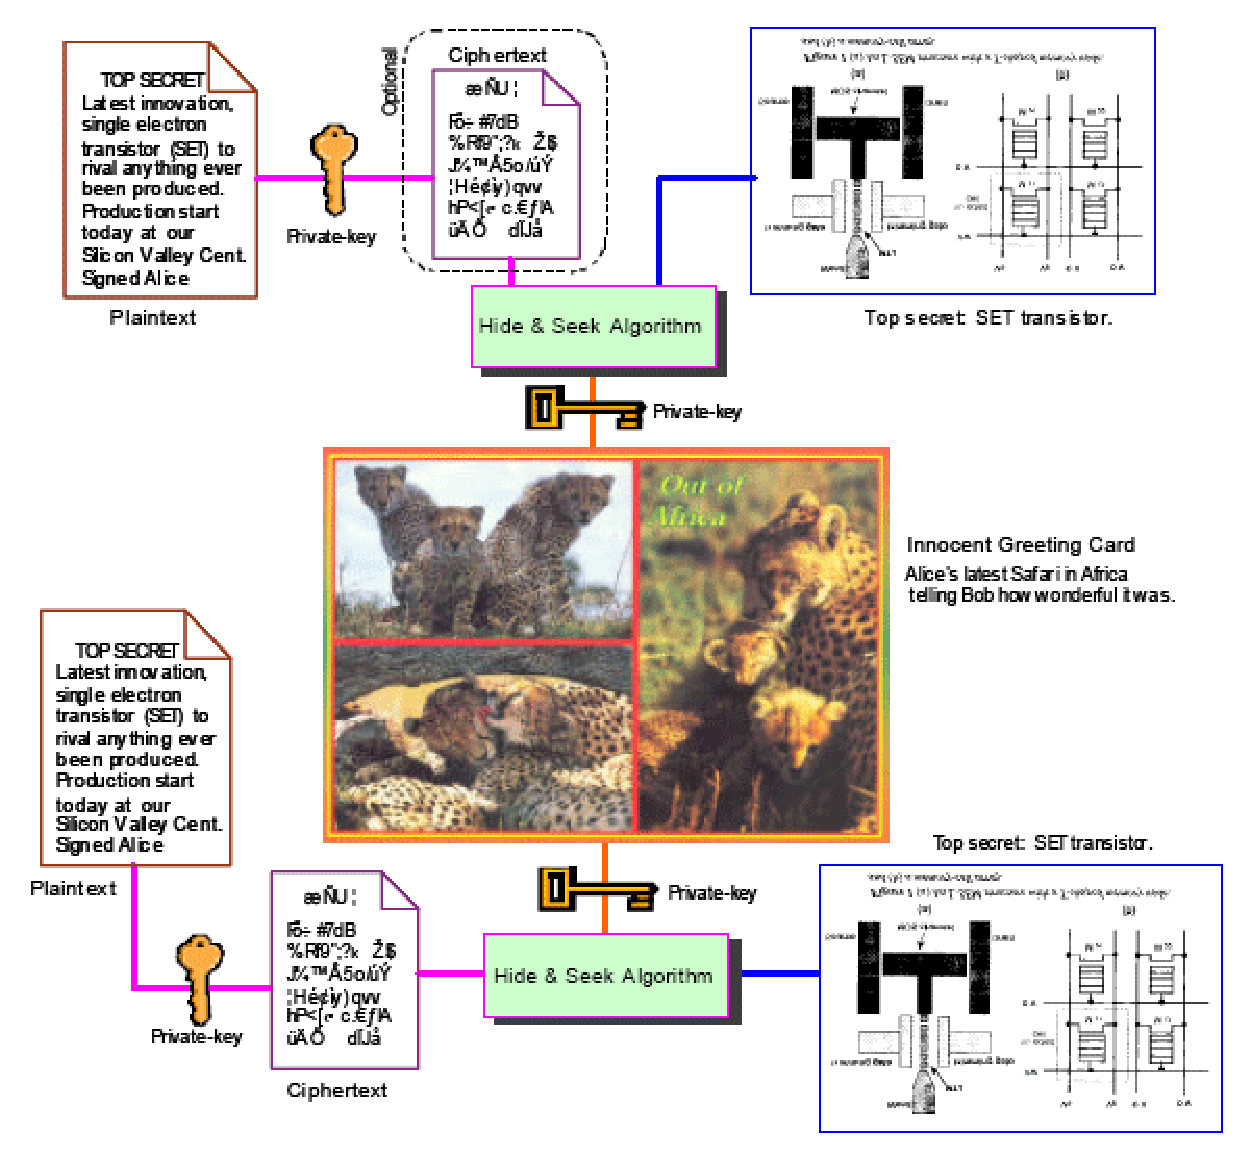
\includegraphics[scale=.25]{images/appli.eps}
			\end{figure}
		\end{itemize}
	\phantom{\cite{CoursUM2, PrincipMax, applidwt, Patch, ARL-TR-1698, DWT-RGB, DWT-DCT, VariousStego, Ondelettes, dwt2doc, applidwt, ClusterStega}}
	\end{frame}
	
	
	\placelogotrue

	
	%%%%%%%% BIBLIOGRAPHY
	
	\begin{frame}[allowframebreaks]{Références}
		\footnotesize
		\bibliographystyle{abbrv}
		\bibliography{refs}
	\end{frame}

\end{document}






